% This text is proprietary.
% It's a part of presentation made by myself.
% It may not used commercial.
% The noncommercial use such as private and study is free
% May 2007
% Author: Sascha Frank 
% University Freiburg 
% www.informatik.uni-freiburg.de/~frank/
%
% 
\documentclass{beamer}
\setbeamertemplate{navigation symbols}{}

\usepackage{beamerthemeshadow}
\usepackage{algorithm}
\usepackage{float}
\usepackage{algpseudocode}

\begin{document}
\title{Evaluation of hill climbing, simulated annealing, tabu search and random selection: search algorithms
       on cryptographic hash functions BLAKE, Gr{\o}stl and Keccak}  
\author{Soham Sadhu}
\date{\today} 

\begin{frame}
\titlepage
\end{frame}

\begin{frame}
\frametitle{Abstract}
\begin{itemize}
\item In October 2012, Keccak was chosen as the winner of SHA-3 competition amongst 64 candidates, including 
the finalists BLAKE and Gr{\o}stl.
\item I have attempted to find near collisions in reduced versions of BLAKE, Gr{\o}stl and Keccak; using hill
climbing, random selection, simulated annealing and tabu search.
\end{itemize}
\end{frame}

\begin{frame}
\frametitle{Table of contents}
\tableofcontents
\end{frame} 

\section{Introduction}

\subsection{Hash function}
\begin{frame}
  \frametitle{Hash function}
  A \emph{hash family} is a four-tuple ($\mathcal{X}, \mathcal{Y}, \mathcal{K}, \mathcal{H}$),
  satisfying the following conditions.\footnotemark
  \begin{itemize}
    \item $\mathcal{X}$ is a set of possible messages
    \item $\mathcal{Y}$ is a finite set of hash function output
    \item $\mathcal{K}$, the \emph{keyspace}, is a finite set of possible keys
    \item For each $K \in \mathcal{K}$, there is a hash function $h_{k} \in \mathcal{H}$. Each 
      $h_{k}: \mathcal{X} \to \mathcal{Y}$ 
  \end{itemize}
  \footnotetext[1]{Douglas R. Stinson. Cryptography Theory and Practice, chapter 4. Cryptographic
  Hash Functions. Chapman \& Hall/CRC, Boca Raton, FL 33487-2742, USA, third edition, 2006.}
\end{frame}

\subsection{Property of hash function}
\begin{frame}
  \frametitle{Property of Hash function\footnotemark}
  \begin{enumerate}
  \item {\bf Preimage resistance} \\
  {\bf Given:} A hash function $h : \mathcal{X} \to \mathcal{Y}$ and an element $y \in \mathcal{Y}$. \\
  {\bf Find:} $x \in \mathcal{X}$ such that $h(x) = y$.
  \item {\bf Second preimage} \\
  {\bf Given:} A hash function $h : \mathcal{X} \to \mathcal{Y}$ and an element $x \in \mathcal{X}$. \\
  {\bf Find:} $x' \in \mathcal{X}$ such that $x' \neq x$ and $h(x) = h(x')$.
  \item {\bf Collision resistance} \\
  {\bf Given:} A hash function $h : \mathcal{X} \to \mathcal{Y}$ \\
  {\bf Find:} $x, x' \in \mathcal{X}$ such that $x' \neq x$ and $h(x') = h(x)$. 
  \end{enumerate}
  \footnotetext[2]{Douglas R. Stinson. Cryptography Theory and Practice, chapter 4. Cryptographic
  Hash Functions. Chapman \& Hall/CRC, Boca Raton, FL 33487-2742, USA, third edition, 2006.}
\end{frame}

\subsection{Security model}
\begin{frame}
\frametitle{Security model}
\begin{itemize}
\item {\bf Random Oracle} model, proposed by Bellare and Rogaway. Algorithm is secure, modulo the way it creates
the random outputs.\footnotemark
\item {\bf Birthday paradox:} In a sample size of $M$, minimum $N$ number of attempts to find, two elements with
same value is given by equation $N \approx 1.17 \sqrt{M}$. 
\end{itemize}
\footnotetext[3]{Gerrit Bleumer. Random oracle model. In HenkC.A. van Tilborg and Sushil Jajodia,
editors, Encyclopedia of Cryptography and Security, pages 1027–1028. Springer US, 2011.}
\end{frame}

\subsection{Application}
\begin{frame}
\frametitle{Application of hash functions}
\begin{enumerate}
\item {\bf Digital forensics:} take a hash value of evidence, to later prove that it has not been tampered.
\footnotemark
\item {\bf Password stored:} is salted and hashed, before inserting to database.
\item {\bf File integrity:} take hash value of files between time intervals, to make sure; they have not
been tampered.
\item {\bf Pseudo random:} generator, based on a seed value.
\end{enumerate}
\footnotetext[4]{Richard P. Salgado. Fourth Amendment Search And The Power Of The Hash, volume
119 of 6, pages 38 – 46. Harvard Law Review Forum, 2006.}
\end{frame}

\subsection{Standards and SHA-3 competition}

\begin{frame}
\frametitle{SHA-0}
\begin{itemize}
\item SHA-0 proposed by NSA in 1993, later standardised by NIST. 
\item In 1995 Florent Chabaud and Antoine Joux, found collisions in SHA-0 with complexity of $2^{61}$.
\item In 2004, Eli Biham and Chen found near collisions for SHA-0, about 142 out of 160 bits to be equal.
\item Full collisions were also found, when the number of rounds for the algorithm were reduced from 80 to 62.
\end{itemize}
\end{frame}

\begin{frame}
\frametitle{SHA-1}
\begin{itemize}
\item In 1995, SHA-0 replaced by SHA-1, designed by NSA\footnotemark. SHA-1 had block size of 512 bits, size of 
160 bits; and additional circular shift operation, to rectify weakness from SHA-0.
\item In 2005, team from Shandong University found collisions on full version of SHA-1 requiring $2^{69}$ 
operations\footnotemark.
\end{itemize}
\footnotetext[5]{James Joshi. Network Security: Know It All: Know It All. Newnes Know It All. Elsevier Science, 2008.}
\footnotetext[6]{Bruce Schneier. Sha-1 broken.
http://www.schneier.com/blog/archives/2005/02/sha1\_broken.html, February 2005.}
\end{frame}

\begin{frame}
\frametitle{SHA-2}
\begin{itemize}
\item SHA-2 was designed by NSA, and released in 2001 by NIST. Family of functions of SHA-224, SHA-256, 
SHA-384, SHA-512.
\item Computational operations for finding collisions in SHA-256 for 23-step was found to be around 
$2^{11.5}$, and for 24 step was $2^{28.5}$ respectively.
\item Computational operations for finding collisions in SHA-512 for 23-step was found to be around 
$2^{16.5}$, and for 24 step was $2^{32.5}$ respectively\footnotemark.
\end{itemize}
\footnotetext[7]{Somitra Kumar Sanadhya and Palash Sarkar. New collision attacks against up to 24-
step sha-2. In Dipanwita Roy Chowdhury, Vincent Rijmen, and Abhijit Das, editors, INDOCRYPT, volume 5365 
of Lecture Notes in Computer Science, pages 91–103. Springer, 2008.}
\end{frame}

\begin{frame}
\frametitle{SHA-3}
\begin{itemize}
\item NIST announced competition for choosing SHA-3 on November, 2007. Entries accepted till October, 2008.
\item 51 candidates from 64 submissions, were accepted for first round on December 9, 2008.
\item Out of 5 finalists, on October 2, 2012; Keccak was announced winner amongst other four finalist, which
included BLAKE and Gr{\o}stl.
\item Keccak was chosen for large security margin, flexibility, and efficient hardware implementation.
\end{itemize}
\end{frame}

\section{SHA-3 finalists}

\subsection{BLAKE}

\begin{frame}
\frametitle{Properties of BLAKE hash function}
\begin{table}[h]
  \begin{center}
    \begin{tabular}{ *{6}{c} } \hline
      Algorithm & Word & Message    & Block & Digest & Salt \\ \hline
      BLAKE-224 & 32   & $< 2^{64}$  & 512   & 224    & 128  \\
      BLAKE-256 & 32   & $< 2^{64}$  & 512   & 256    & 128  \\
      BLAKE-384 & 64   & $< 2^{128}$ & 1024  & 384    & 256  \\
      BLAKE-512 & 64   & $< 2^{128}$ & 1024  & 512    & 256  \\ \hline
    \end{tabular}
    \caption{Specification of available input, output, block and salt sizes for various BLAKE hash functions,
    size in bits. \footnotemark}
  \end{center}
\end{table}
\footnotetext[9]{Jean-Philippe Aumasson, Luca Henzen, Willi Meier, and Raphael C.-W. Phan. Blake.
http://www.131002.net/blake/blake.pdf, April 2012.}
\end{frame}

\begin{frame}
\frametitle{BLAKE construction}
BLAKE is built on HAIFA (HAsh Iterative FrAmework) structure \footnotemark which is an improved version of 
Merkle-Damg\.{a}rd function.
\begin{figure}[h]
  \begin{center}
    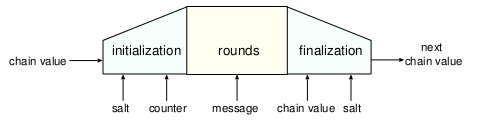
\includegraphics[scale=0.5]{blakelocalwidepipeconstruction.jpg}
  \end{center}
  \caption{Local wide construction of BLAKE's compression function\footnotemark}
  \label{fig:seq}
\end{figure}
\footnotetext[10]{Eli Biham and Orr Dunkelman. A framework for iterative hash functions - haifa.
Cryptology ePrint Archive, Report 2007/278, 2007.}
\footnotetext[11]{Jean-Philippe Aumasson, Luca Henzen, Willi Meier, and Raphael C.-W. Phan. Blake.
http://www.131002.net/blake/blake.pdf, April 2012.}
\end{frame}

\begin{frame}
\frametitle{Padding rule}
\begin{itemize}
\item For variant producing digest size 224, 256 input message is padded with '1' followed by '0' bits,
so that length is 447 modulo 512. Followed by bit '1', and 64 bit unsigned big endian representation 
of block length. 
\item For variant producing digest size 384, 512 input message is padded by bit '1', followed by '0' bits
till length is 895 modulo 1024. Followed by bit '1', and 128 bit unsigned big endian representation of 
block length in bits.
\end{itemize}
\end{frame}

\begin{frame}[fragile]
\frametitle{Compression algorithm}
  \begin{algorithm}[H]
  \begin{algorithmic}[1]
    \State $ h^{0} \gets IV $
    \For {$i = 0,\dots, N - 1$}
      \State $h^{i+1} \gets compress(h^{i}, m^{i}, s, l^{i})$
    \EndFor
    \State\Return{$h^{N}$}
  \end{algorithmic}
  \caption[BLAKE Compression]{BLAKE Compression procedure\footnotemark}
  \label{alg:seq}
  \end{algorithm}
  \footnotetext[12]{Jean-Philippe Aumasson, Luca Henzen, Willi Meier, and Raphael C.-W. Phan. Blake.
http://www.131002.net/blake/blake.pdf, April 2012.}
\end{frame}

\begin{frame}
\frametitle{Initialization of the state}
\begin{center}
$\begin{pmatrix} v_{0} & v_{1} & v_{2} & v_{3} \\ v_{4} & v_{5} & v_{6} & v_{7} \\
                 v_{8} & v_{9} & v_{10} & v_{11} \\ v_{12} & v_{13} & v_{14} & v_{15}\end{pmatrix} 
\gets
\begin{pmatrix} h_{0} & h_{1} & h_{2} & h_{3} \\ h_{4} & h_{5} & h_{6} & h_{7} \\
   s_{0} \oplus c_{0} & s_{1} \oplus c_{1} & s_{2} \oplus c_{2} & s_{3} \oplus c_{3} \\ 
   t_{0} \oplus c_{4} & t_{0} \oplus c_{5} & t_{1} \oplus c_{6} & t_{1} \oplus c_{7} \end{pmatrix}$
\end{center}
After initialization the matrix is operated for 14 or 16 rounds depending on version, on the following 
groups represented as $G_{i}(a, b, c, d)$
\begin{table}
  \begin{center}
    \begin{tabular}{ *{3}{c}}
    $ G_{0}(v_{0}, v_{8}, v_{12})$ & $G_{1}(v_{1}, v_{5}, v_{9}, v_{13})$ & $G_{2}(v_{2}, v_{6}, v_{10}, v_{14})$ \\
    $G_{3}(v_{3}, v_{7}, v_{11}, v_{15}) $ & $G_{4}(v_{0}, v_{5}, v_{10}, v_{15})$ & $G_{5}(v_{1}, v_{6}, v_{11}, v_{12})$ \\
    $G_{6}(v_{2}, v_{7}, v_{8}, v_{13})$ & $G_{7}(v_{3}, v_{4}, v_{9}, v_{14})$
    \end{tabular}
  \end{center}
\end{table}
\end{frame}

\begin{frame}
\frametitle{BLAKE permutation operation for 224 and 256 variant}
$a \gets a + b + (m_{\sigma_{r}(2i)} \oplus c_{\sigma_{r}(2i + 1)}) $ \\
$d \gets (d \oplus a) \ggg 16$ \\
$c \gets c + d$ \\
$b \gets (b \oplus c) \ggg 12$ \\
$a \gets a + b + (m_{\sigma_{r}(2i + 1)} \oplus c_{\sigma_{r}(2i)})$ \\
$d \gets (d \oplus a) \ggg 8$ \\
$c \gets c + d$ \\
$b \gets (b \oplus c) \ggg 7$ \\ 
\noindent\rule{10cm}{0.4pt} \\
\vspace{1mm}
+ addition in modulo $2^{32}$ \\
$\ggg k$ rotate to right by k bits \\
$\oplus$ bitwise XOR \\
r permutation round \\
i is from $G_{i}$
\end{frame}

\begin{frame}
\frametitle{Permutation round selection, $\sigma$ function\footnotemark}
  \resizebox{\linewidth}{!} {
    \begin{tabular}{ c| *{16}{c}} \hline
      $\sigma_{0}$ & 0  & 1  & 2  & 3  & 4  & 5  & 6  & 7  & 8  & 9  & 10 & 11 & 12 & 13 & 14 & 15 \\
      $\sigma_{1}$ & 14 & 10 & 4  & 8  & 9  & 15 & 13 & 6  & 1  & 12 & 0  & 2  & 11 & 7  & 5  & 3  \\
      $\sigma_{2}$ & 11 & 8  & 12 & 0  & 5  & 2  & 15 & 13 & 10 & 14 & 3  & 6  & 7  & 1  & 9  & 4  \\
      $\sigma_{3}$ & 7  & 9  & 3  & 1  & 13 & 12 & 11 & 14 & 2  & 6  & 5  & 10 & 4  & 0  & 15 & 8  \\
      $\sigma_{4}$ & 9  & 0  & 5  & 7  & 2  & 4  & 10 & 15 & 14 & 1  & 11 & 12 & 6  & 8  & 3  & 13 \\
      $\sigma_{5}$ & 2  & 12 & 6  & 10 & 0  & 11 & 8  & 3  & 4  & 13 & 7  & 5  & 15 & 14 & 1  & 9  \\
      $\sigma_{6}$ & 12 & 5  & 1  & 15 & 14 & 13 & 4  & 10 & 0  & 7  & 6  & 3  & 9  & 2  & 8  & 11 \\
      $\sigma_{7}$ & 13 & 11 & 7  & 14 & 12 & 1  & 3  & 9  & 5  & 0  & 15 & 4  & 8  & 6  & 2  & 10 \\
      $\sigma_{8}$ & 6  & 15 & 14 & 9  & 11 & 3  & 0  & 8  & 12 & 2  & 13 & 7  & 1  & 4  & 10 & 5  \\
      $\sigma_{9}$ & 10 & 2  & 8  & 4  & 7  & 6  & 1  & 5  & 15 & 11 & 9  & 14 & 3  & 12 & 13 & 0  \\ \hline
    \end{tabular}
  }
  \footnotetext[13]{Jean-Philippe Aumasson, Luca Henzen, Willi Meier, and Raphael C.-W. Phan. Blake.
http://www.131002.net/blake/blake.pdf, April 2012.}
\end{frame}

\begin{frame}
\frametitle{BLAKE permutation operation for 384 and 512 variant}
$a \gets a + b + (m_{\sigma_{r}(2i)} \oplus c_{\sigma_{r}(2i + 1)})$ \\
$d \gets (d \oplus a) \ggg 32$ \\
$c \gets c + d$ \\
$b \gets (b \oplus c) \ggg 25$ \\
$a \gets a + b + (m_{\sigma_{r}(2i + 1)} \oplus c_{\sigma_{r}(2i)})$ \\
$d \gets (d \oplus a) \ggg 16$ \\
$c \gets c + d$ \\
$b \gets (b \oplus c) \ggg 11$ \\
\noindent\rule{10cm}{0.4pt} \\
\vspace{1mm}
+ addition in modulo $2^{64}$ \\
\end{frame}

\begin{frame}
\frametitle{Finalization}
$h'_{0} \gets h_{0} \oplus s_{0} \oplus v_{0} \oplus v_{8}$ \\
$h'_{1} \gets h_{1} \oplus s_{1} \oplus v_{1} \oplus v_{9}$ \\
$h'_{2} \gets h_{2} \oplus s_{2} \oplus v_{2} \oplus v_{10}$ \\
$h'_{3} \gets h_{3} \oplus s_{3} \oplus v_{3} \oplus v_{11}$ \\
$h'_{4} \gets h_{4} \oplus s_{0} \oplus v_{4} \oplus v_{12}$ \\
$h'_{5} \gets h_{5} \oplus s_{1} \oplus v_{5} \oplus v_{13}$ \\
$h'_{6} \gets h_{6} \oplus s_{2} \oplus v_{6} \oplus v_{14}$ \\
$h'_{7} \gets h_{7} \oplus s_{3} \oplus v_{7} \oplus v_{15}$ \\
\end{frame}

\subsection{Gr{\o}stl}

\begin{frame}
\frametitle{Padding}
\begin{itemize}
\item The message is split into blocks of 512 bits for variants of digest size upto 256 bits; and into 1024 bit
block for variant of digest size above 256 bits.
\item Bit '1' is appended, then $ w = -N - 65 \thickspace mod \thickspace l $, 0 bits are appended; followed by
64 bit representation of $(N + w + 65) / l $.
\item Due to encoding of message in padded block, the maximum size of message for short variants is $2^{73}-577$
bits, and that for variants above 256 is $2^{74}-1089$bits.
\end{itemize}
\end{frame}

\begin{frame}
\frametitle{Initial values and rounds \footnotemark}
\begin{table}[h]
  \begin{center}
    \begin{tabular}{ *{3}{c} } \hline
      Permutations            & Digest size & Recommended value of r \\ \hline
      $P_{512}$ and $Q_{512}$   & 8 - 256     & 10 \\
      $P_{1024}$ and $Q_{1024}$ & 264 - 512   & 14 \\ \hline 
    \end{tabular}
    \caption{Recommended number of rounds}
  \end{center}
\end{table}

\begin{table}[h]
  \begin{center}
    \begin{tabular}{ *{2}{c} } \hline
      n   & $iv_{n}$         \\ \hline
      224 & 00 $\dots$ 00 00 e0 \\
      256 & 00 $\dots$ 00 01 00 \\
      384 & 00 $\dots$ 00 01 80 \\
      512 & 00 $\dots$ 00 02 00 \\ \hline
    \end{tabular}
  \caption{Initial values for Gr{\o}stl-n function.}
  \end{center}
\end{table}
\footnotetext[14]{S{\o}ren Steffen Thomsen, Martin Schl\"{a}ffer, Christian Rechberger, Florian Mendel,
Krystian Matusiewicz, Lars R. Knudsen, and Praveen Gauravaram. Grøstl - a sha-3
candidate version 2.0.1. http://www.groestl.info/Groestl.pdf, March 2011.}
\end{frame}

\begin{frame}
\frametitle{Hashing the message}
After padding, the message is broken to blocks, and processed sequentially. An initial $h_{0}$ = iv is defined.
\begin{center}$ h_{i}\gets f(h_{i-1}, m_{i})\thickspace for \thickspace i = 1,\ldots, t.$\end{center}
\begin{figure}
  \begin{center}
    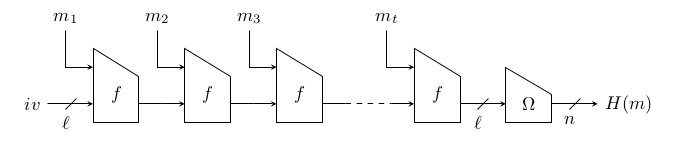
\includegraphics[scale=0.5]{groestlhashfunction.jpg}
  \end{center}
  \caption{Gr{\o}stl hash function \footnotemark}
  \label{fig:lab}
\end{figure}
\footnotetext[15]{S{\o}ren Steffen Thomsen, Martin Schl\"{a}ffer, Christian Rechberger, Florian Mendel,
Krystian Matusiewicz, Lars R. Knudsen, and Praveen Gauravaram. Grøstl - a sha-3
candidate version 2.0.1. http://www.groestl.info/Groestl.pdf, March 2011.}
\end{frame}

\begin{frame}
\frametitle{Input mapping}
Mapping of the input bytes to the state in following order. \\
\vspace{3mm}
$\begin{bmatrix}
  00 & 08 & 10 & 18 & 20 & 28 & 30 & 38 \\
  01 & 09 & 11 & 19 & 21 & 29 & 31 & 39 \\
  02 & 0a & 12 & 1a & 22 & 2a & 32 & 3a \\
  03 & 0b & 13 & 1b & 23 & 2b & 33 & 3b \\
  04 & 0c & 14 & 1c & 24 & 2c & 34 & 3c \\
  05 & 0d & 15 & 1d & 25 & 2d & 35 & 3d \\
  06 & 0e & 16 & 1e & 26 & 2e & 36 & 3e \\
  07 & 0f & 17 & 1f & 27 & 2f & 37 & 3f
\end{bmatrix}$
\end{frame}

\begin{frame}
\frametitle{Permutation f function}
\begin{center}$f(h, m) = P(h \oplus m) \oplus Q(m) \oplus h.$\end{center}
\begin{figure}[h]
  \begin{center}
    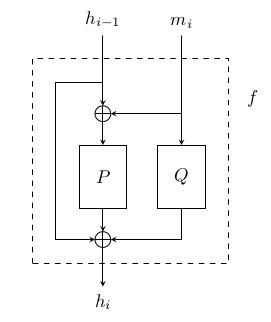
\includegraphics[scale=0.5]{groestlPQfunction.jpg}
  \end{center}
  \caption{Compression functions, where P and Q are $l-bit$ permutations \footnotemark}
  \label{fig:lab}
\end{figure}
\footnotetext[16]{S{\o}ren Steffen Thomsen, Martin Schl\"{a}ffer, Christian Rechberger, Florian Mendel,
Krystian Matusiewicz, Lars R. Knudsen, and Praveen Gauravaram. Grøstl - a sha-3
candidate version 2.0.1. http://www.groestl.info/Groestl.pdf, March 2011.}
\end{frame}

\begin{frame}
\frametitle{Omega truncate function}
The $\Omega$ function consists of a $trunc_{n}(x)$ that outputs only the trailing n bits of input x.
\begin{center}$\Omega(x) = trunc_{n}( P(x) \oplus x ).$\end{center}
\begin{figure}[h]
  \begin{center}
    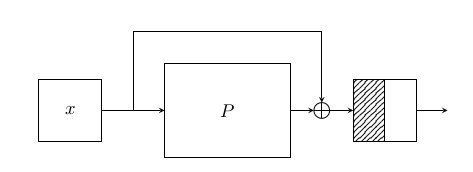
\includegraphics[width=4.5in]{groestlomegafunction.jpg}
  \end{center}
  \caption{Omega truncation function \footnotemark}
  \label{fig:lab}
\end{figure}
\footnotetext[17]{S{\o}ren Steffen Thomsen, Martin Schl\"{a}ffer, Christian Rechberger, Florian Mendel,
Krystian Matusiewicz, Lars R. Knudsen, and Praveen Gauravaram. Grøstl - a sha-3
candidate version 2.0.1. http://www.groestl.info/Groestl.pdf, March 2011.}
\end{frame}

\begin{frame}
\frametitle{Contents of P and Q function}
The P and Q functions are represented by a round, with slight variation in variables they operate.
\begin{center}$ R = MixBytes \cdot ShiftBytes \cdot SubBytes \cdot AddRoundConstant $ \end{center}
\end{frame}

\begin{frame}
\frametitle{Add Round Constant}
$A \gets A \oplus C[i]$ where A is state matrix and C is constant matrix.
$ P_{1024}: C[i] = \begin{bmatrix}
  00 \oplus i & 10 \oplus i & 20 \oplus i \ldots f0 \oplus i \\
  00          & 00          & 00          \dots  00          \\
  \vdots      & \vdots      & \vdots      \dots  \vdots      \\
\end{bmatrix}$

and 

$Q_{1024}: C[i] = \begin{bmatrix}
  ff          & ff          & ff          \dots ff          \\
  \vdots      & \vdots      & ff          \dots ff          \\
  ff \oplus i & ef \oplus i & df \oplus i \dots 0f \oplus i
\end{bmatrix}$
\end{frame}

\begin{frame}
\frametitle{Substitute byte}
$a_{i,j} \gets S( a_{i,j}),  0 \leq i < 8, 0 \leq j < v.$ 
\resizebox{\linewidth}{!} {
    \begin{tabular}{ c | *{16}{c}}
     & 00 & 01 & 02 & 03 & 04 & 05 & 06 & 07 & 08 & 09 & 0a & 0b & 0c & 0d & 0e & 0f \\ \hline
  00 & 63 & 7c & 77 & 7b & f2 & 6b & 6f & c5 & 30 & 01 & 67 & 2b & fe & d7 & ab & 76 \\ 
  10 & ca & 82 & c9 & 7d & fa & 59 & 47 & f0 & ad & d4 & a2 & af & 9c & a4 & 72 & c0 \\
  20 & b7 & fd & 93 & 26 & 36 & 3f & f7 & cc & 34 & a5 & e5 & f1 & 71 & d8 & 31 & 15 \\
  30 & 04 & c7 & 23 & c3 & 18 & 96 & 05 & 9a & 07 & 12 & 80 & e2 & eb & 27 & b2 & 75 \\
  40 & 09 & 83 & 2c & 1a & 1b & 6e & 5a & a0 & 52 & 3b & d6 & b3 & 29 & e3 & 2f & 84 \\
  50 & 53 & d1 & 00 & ed & 20 & fc & b1 & 5b & 6a & cb & be & 39 & 4a & 4c & 58 & cf \\
  60 & d0 & ef & aa & fb & 43 & 4d & 33 & 85 & 45 & f9 & 02 & 7f & 50 & 3c & 9f & a8 \\
  70 & 51 & a3 & 40 & 8f & 92 & 9d & 38 & f5 & bc & b6 & da & 21 & 10 & ff & f3 & d2 \\
  80 & cd & 0c & 13 & ec & 5f & 97 & 44 & 17 & c4 & a7 & 7e & 3d & 64 & 5d & 19 & 73 \\
  90 & 60 & 81 & 4f & dc & 22 & 2a & 90 & 88 & 46 & ee & b8 & 14 & de & 5e & 0b & db \\
  a0 & e0 & 32 & 3a & 0a & 49 & 06 & 24 & 5c & c2 & d3 & ac & 62 & 91 & 95 & e4 & 79 \\
  b0 & e7 & c8 & 37 & 6d & 8d & d5 & 4e & a9 & 6c & 56 & f4 & ea & 65 & 7a & ae & 08 \\
  c0 & ba & 78 & 25 & 2e & 1c & a6 & b4 & c6 & e8 & dd & 74 & 1f & 4b & bd & 8b & 8a \\
  d0 & 70 & 3e & b5 & 66 & 48 & 03 & f6 & 0e & 61 & 35 & 57 & b9 & 86 & c1 & 1d & 9e \\
  e0 & e1 & f8 & 98 & 11 & 69 & d9 & 8e & 94 & 9b & 1e & 87 & e9 & ce & 55 & 28 & df \\
  f0 & 8c & a1 & 89 & 0d & bf & e6 & 42 & 68 & 41 & 99 & 2d & 0f & b0 & 54 & bb & 16 \\
  \end{tabular}
  }
\end{frame}

\begin{frame}
\frametitle{Shift byte}
\begin{figure}[h]
  \begin{center}
    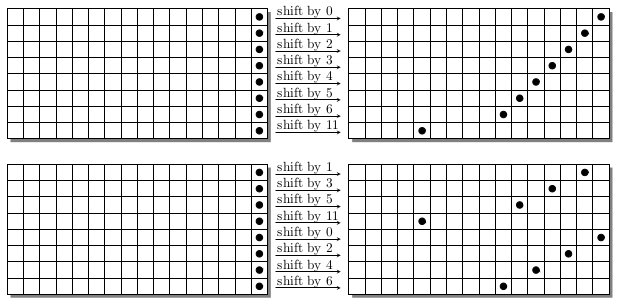
\includegraphics[scale=0.5]{groestl1024shift.jpg}
  \end{center}
  \caption{ShiftBytes transformation of permutation $P_{1024}$(top) and $Q_{1024}$(bottom)\footnotemark}
  \label{fig:lab}
\end{figure}
\footnotetext[18]{S{\o}ren Steffen Thomsen, Martin Schl\"{a}ffer, Christian Rechberger, Florian Mendel,
Krystian Matusiewicz, Lars R. Knudsen, and Praveen Gauravaram. Grøstl - a sha-3
candidate version 2.0.1. http://www.groestl.info/Groestl.pdf, March 2011.}
\end{frame}

\begin{frame}
\frametitle{Mix byte}
$ A \gets B \times A$ \\
B is a finite field over $\mathbb{F}_{256}$, 
defined over $\mathbb{F}_{2}$ by polynomial $x^{8} \oplus x^{4} \oplus x^{3} \oplus x \oplus 1$. \\
\vspace{3mm}
$B = \begin{bmatrix}
02 & 02 & 03 & 04 & 05 & 03 & 05 & 07 \\
07 & 02 & 02 & 03 & 04 & 05 & 03 & 05 \\
05 & 07 & 02 & 02 & 03 & 04 & 05 & 03 \\
03 & 05 & 07 & 02 & 02 & 03 & 04 & 05 \\
05 & 03 & 05 & 07 & 02 & 02 & 03 & 04 \\
04 & 05 & 03 & 05 & 07 & 02 & 02 & 03 \\
03 & 04 & 05 & 03 & 05 & 07 & 02 & 02 \\
02 & 03 & 04 & 05 & 03 & 05 & 07 & 02 \\
\end{bmatrix}$
\end{frame}

\subsection{Keccak}

\begin{frame}
\frametitle{Keccak sponge construction}
\begin{figure}[h]
  \begin{center}
    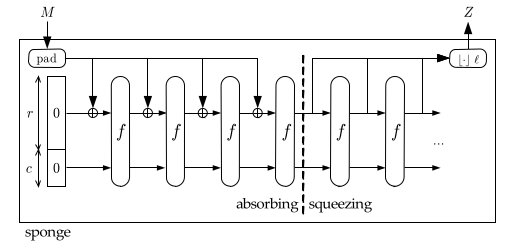
\includegraphics[scale=0.5]{keccakspongeconstruction.jpg}
  \end{center}
  \caption{Sponge construction $Z = Sponge[f, pad, r](M, l)$\footnotemark}
  \label{fig:lab}
\end{figure}
\footnotetext[21]{Guido Bertoni, Joan Daemen, Micha\"{e}l Peeters, and Gilles Van Assche. Cryptographic
sponge functions. http://sponge.noekeon.org/CSF-0.1.pdf, January 2011.}
\end{frame}

\begin{frame}
\frametitle{Keccak state}
\begin{figure}[h]
  \begin{center}
    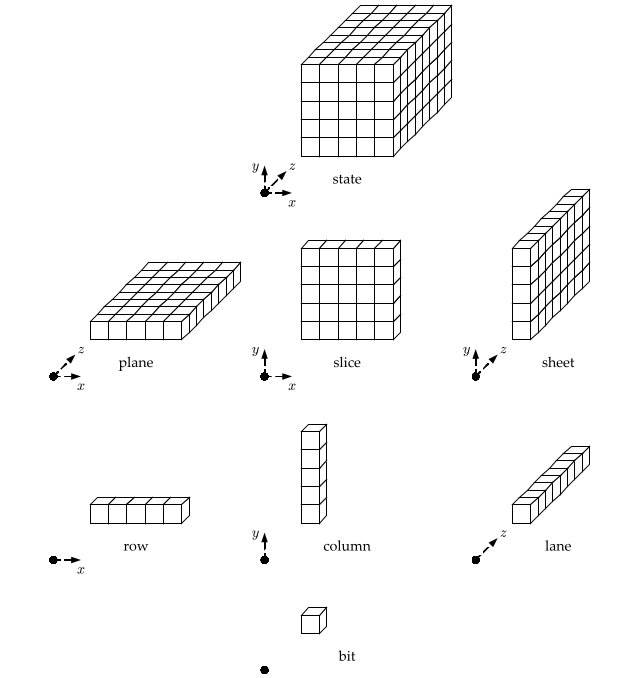
\includegraphics[scale=0.25]{keccakstateterminology.jpg}
  \end{center}
  \caption{Keccak state terminology $Z = Sponge[f, pad, r](M, l)$\footnotemark}
  \label{fig:lab}
\end{figure}
\footnotetext[22]{Guido Bertoni, Joan Daemen, Micha\"{e}l Peeters, and Gilles Van Assche. The keccak 
reference. http://keccak.noekeon.org/Keccak-reference-3.0.pdf, January 2011.}
\end{frame}

\begin{frame}
\frametitle{Padding and permutations}
\begin{itemize}
\item The message is padded with $1 0^{*}1$ to make it multiple of the block length.
\item $R = \iota \circ \chi \circ \pi \circ \rho \circ \theta$
\item The permutation round R is repeated for 12 + 2l times, where l is the lane length. The default
capacity size is 576.
\end{itemize}
\end{frame}

\begin{frame}
\frametitle{Contents of Keccak permutation round}
\begin{align*}
  \theta &: a[x][y][z] & \gets & \thickspace a[x][y][z] + \displaystyle\sum\limits_{y' = 0}^{4} a[x - 1][y'][z] + \displaystyle\sum\limits_{y' = 0}^{4} a[x + 1][y'][z - 1], \\
  \rho &: a[x][y][z] & \gets & \thickspace a[x][y][z - (t + 1)(t + 2) / 2], \\
  & & & \thickspace t \thickspace satisfying \thickspace 0 \leq t < 24 \thickspace and \thickspace
  \begin{pmatrix} 0 & 1 \\ 2 & 3 \end{pmatrix}^{t} \begin{pmatrix} 1 \\ 0 \end{pmatrix} = \begin{pmatrix} x \\ y \end{pmatrix}
  in \thickspace GF(5)^{2 \times 2}, \\
  & & & \thickspace or \thickspace t = -1 \thickspace if \thickspace x = y = 0, \\
  \pi &: a[x][y] & \gets & \thickspace a[x'][y'], \thickspace with \thickspace
  \begin{pmatrix} x \\ y \end{pmatrix} = \begin{pmatrix} 0 & 1 \\ 2 & 3 \end{pmatrix} \begin{pmatrix} x' \\ y'\end{pmatrix}, \\
  \chi &: a[x] & \gets & \thickspace a[x] + (a[x + 1] + 1) \thickspace a[x + 2], \\
  \iota &: a & \gets & \thickspace a + RC[i_{r}].
\end{align*}
\end{frame}

\begin{frame}
\frametitle{$\theta$ step}
\begin{figure}[h]
  \begin{center}
    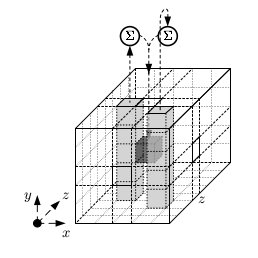
\includegraphics[scale=0.5]{keccaktheta.jpg}
  \end{center}
  \caption{$\theta$ applied to a single row\footnotemark}
  \label{fig:lab}
\end{figure}
\footnotetext[23]{Guido Bertoni, Joan Daemen, Micha\"{e}l Peeters, and Gilles Van Assche. The keccak 
reference. http://keccak.noekeon.org/Keccak-reference-3.0.pdf, January 2011.}
\end{frame}

\begin{frame}
\frametitle{$\rho$ step}
\begin{figure}[h]
  \begin{center}
    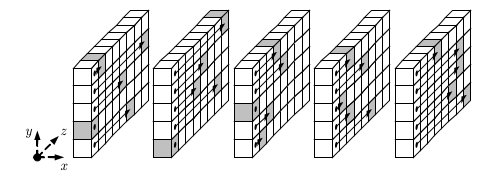
\includegraphics[scale=0.5]{keccakrho.jpg}
  \end{center}
  \caption{$\rho$ transformation applied to lanes\footnotemark}
  \label{fig:lab}
\end{figure}
\footnotetext[24]{Guido Bertoni, Joan Daemen, Micha\"{e}l Peeters, and Gilles Van Assche. The keccak 
reference. http://keccak.noekeon.org/Keccak-reference-3.0.pdf, January 2011.}
\end{frame}

\begin{frame}
\frametitle{$\pi$ step}
\begin{figure}[h]
  \begin{center}
    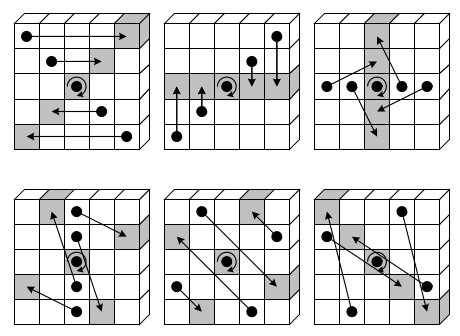
\includegraphics[scale=0.35]{keccakpi.jpg}
  \end{center}
  \caption{$\pi$ applied to a single slice\footnotemark}
  \label{fig:lab}
\end{figure}
\footnotetext[25]{Guido Bertoni, Joan Daemen, Micha\"{e}l Peeters, and Gilles Van Assche. The keccak 
reference. http://keccak.noekeon.org/Keccak-reference-3.0.pdf, January 2011.}
\end{frame}

\begin{frame}
\frametitle{$\chi$ step}
\begin{figure}[h]
  \begin{center}
    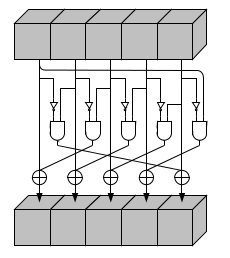
\includegraphics[scale=0.35]{keccakchi.jpg}
  \end{center}
  \caption{$\chi$ applied to a single row.\footnotemark}
  \label{fig:lab}
\end{figure}
\footnotetext[26]{Guido Bertoni, Joan Daemen, Micha\"{e}l Peeters, and Gilles Van Assche. The keccak 
reference. http://keccak.noekeon.org/Keccak-reference-3.0.pdf, January 2011.}
\end{frame}

\begin{frame}
\frametitle{$\iota$ step}
\begin{itemize}
\item The round constants are given by
\begin{center}$RC[i_{r}][0][0][2^{j} - 1] = rc[j + 7i_{r}]$ for all $ 0 \leq j \leq l$,\end{center}
\item $rc[t] = (x^{t} \thickspace mod \thickspace x^{8} + x^{6} + x^{5} + x^{4} + 1)$ mod x in GF(2)[$x$]
\end{itemize}
\end{frame}

\section{Related work, hypothesis based on hill climbing}

\subsection{Rotational cryptanalysis of reduced round Keccak}

\begin{frame}
\frametitle{Rotational cryptanalysis in ARX}
\begin{itemize}
\item Rotational cryptanalysis that studies propogation of rotational pair throug a primitive, is used on 
reduced version of Threefish, a core of Skein\footnotemark.
\item Pair of two 1600-bit states $(A, A^{\leftarrow})$ are called rotational pair when each lane in 
state $A^{\leftarrow}$ is created by bitwise rotation of operation of corresponding lane in state $A$
\footnotemark.
\end{itemize}
\footnotetext[27]{Dmitry Khovratovich and Ivica Nikoli. Rotational cryptanalysis of arx. In Seokhie
Hong and Tetsu Iwata, editors, Fast Software Encryption, volume 6147 of Lecture
Notes in Computer Science, pages 333–346. Springer Berlin Heidelberg, 2010.}
\footnotetext[28]{Pawe{\l} Morawiecki, Josef Pieprzyk, and Marian Srebrny. Rotational cryptanalysis of
round-reduced keccak. Cryptology ePrint Archive, Report 2012/546, 2012. http://eprint.iacr.org/2012/546.pdf.}
\end{frame}

\begin{frame}
\frametitle{Definitions}
\begin{enumerate}
\item Set $S_n$ is a set of $2^{1600}$ pairs of states which are created by an operation of KECCAK-f[1600] 
applied to all possible rotational pairs.
\item Probability $p^{n}_{(x, y, z)}$ is the probability for pair of states $(A, A^{\leftarrow})$ randomly 
selected from the set $S_n$ we have $A_{(x, y, z)} = A^{\leftarrow}_{(x, y, z + n)}$.
\item Given probability distribution $\mathcal{D}_n$ that assigns probability $\frac{1}{n!}$ for each 
$p \in \mathcal{P}_n$. A permutation is random, if chosen from $\mathcal{D}_n$.
\end{enumerate}
\end{frame}

\subsection{Hill climbing}
\subsection{Other search algorithms}
\subsection{Hypothesis}

\end{document}
